\documentclass{superfri}
\usepackage[T1]{fontenc}
\usepackage[utf8]{inputenc}
\usepackage{amsmath}
\usepackage{amssymb}
\usepackage{amsthm}
\usepackage[cal=rsfso]{mathalfa}
\usepackage{booktabs}
\usepackage{multirow}
\usepackage{makecell}
\usepackage{tabularx}
\usepackage{float}
\usepackage{algorithm}
\usepackage{algpseudocode}
\usepackage[normalem]{ulem}
\usepackage{graphicx}
\usepackage{xurl} 
\usepackage{lmodern}
\usepackage[unicode=true,linktocpage=true]{hyperref}
\usepackage{type1cm}

\begin{document}


\author{D.\,A.~Grigoriev\footnote{\label{msu}Lomonosov Moscow State University, Moscow, Russia}\footnote{E-mail: dagrig14@yandex.ru}
\and D.\,I.~Chernyshev\footnoteref{msu}\footnote{E-mail: chdanorbis@yandex.ru}}

\title{RuWikiBench: Evaluating Large Language Models through replication of encyclopedia articles}

\maketitle{}

\begin{abstract}
In light of the growing interest in using large language models (LLMs) as tools for generating scientific texts,
the evaluation of their ability to produce encyclopedic content is becoming increasingly relevant.
However, for Russian-language materials this issue has not been sufficiently studied, and existing benchmarks do not cover key aspects of analytical work with sources.
This paper presents RuWikiBench - an open benchmark based on Ruwiki for evaluating the ability of large language models to reproduce Wikipedia-style articles,
built around three tasks:
selection of relevant sources, article structuring, and section generation.
The results of testing popular open-source LLMs show that even under ideal conditions, the best models do not always follow the expert logic of composing encyclopedic content:
even with a perfect source retrieval system, the models cannot reproduce the reference table of contents, and the quality of section generation shows almost no dependence on the number of parameters.

\keywords{benchmark, Wikipedia, Ruwiki, large language model}
\end{abstract}

\section*{Introduction}
Modern large language models demonstrate impressive results in generating texts of various styles and themes. 
However, their capabilities for working with scientific and encyclopedic materials remain understudied, particularly for Russian-language texts. 
Existing methods for evaluating model capabilities predominantly focus on standard linguistic tasks, without paying sufficient attention to analytical abilities when working with scientific texts. 
For the Russian language, this problem is especially relevant due to the limited availability of specialized evaluation tools.

There are many benchmarks covering various linguistic tasks for the Russian language. 
RussianSuperGlue \cite{rsglue} evaluates general language understanding and basic natural language processing tasks. 
MERA \cite{mera} provides unified testing conditions for models by compiling generation instructions for each task; however, the tasks themselves are oriented towards testing general comprehension. 
LIBRA \cite{libra} focuses on testing a model's ability to retain and retrieve information from a large context but is centered on short answers that do not require deep reasoning. 
Ru Arena General \cite{arena} focuses on pairwise model comparison rather than overall answer quality. 
Ping-Pong \cite{pp} evaluates the dialog abilities of models, which is important for interactive systems, but is not suitable for assessing the ability to conduct research and write coherent scientific-encyclopedic texts. 
At the same time, an entire class of tasks related to deep text analysis remains uncovered: creating detailed, structured, and factually accurate texts supported by a large number of sources.

The recent development of new agent capabilities, such as the emergence of the "Deep Research" function by OpenAI \cite{deepr} or the development of the universal Storm algorithm \cite{storm}, 
indicates a growing interest in conducting scientific research using large language models. This highlights the need to create new approaches for objectively evaluating the analytical capabilities of models. 
Existing benchmarks only partially address aspects critical for generating scientific-encyclopedic texts, such as the ability to synthesize information from a set of documents, plan the structure of a future text, 
maintain coherence and logical sequence of presentation, as well as ensure the accuracy and reliability of facts. One of the closest studies in this area is the ResearchArena \cite{resar} benchmark, 
which formalizes the construction of an academic review; however, it is more aimed at testing the models' ability to select and organize relevant information and does not address their ability to generate coherent scientific-encyclopedic texts.

This paper proposes an approach aimed at creating tools to test how well large language models can work with scientific-encyclopedic texts. Within the framework of this research:
\begin{enumerate}
\item A labeled dataset based on the online encyclopedia "Ruwiki" has been collected;
\item An open benchmark, RuWikiBench, has been developed to measure model quality on tasks requiring deep text analysis;
\item The abilities of the best open large language models to generate Wikipedia-style articles have been tested.
\end{enumerate}

The code and data of this work have been made publicly available\footnote{\url{https://github.com/Nejimaki-Tori/WikiBench}}.

\section{Dataset collection}

To build a benchmark aimed at assessing the ability of language models to work with article sources, it is necessary to prepare a corpus of texts that will be used in generation. The choice was made in favor of the Wikipedia style because this genre simultaneously requires factual accuracy, completeness of analysis, and understanding of context, which aligns well with the research direction of this work.

The Russian online encyclopedia "Ruwiki" was chosen as the source. It is distinguished by a large number of references to Russian-language sources, as well as stricter text filtering, which allows it to be relied upon as a reliable benchmark for assessing the quality of generating Russian-language articles.

The data acquisition process included the following steps:

\begin{enumerate}
\item \textbf{Article Selection}: Articles on diverse topics containing a sufficient number of references to external sources were manually selected;
\item \textbf{Source Downloading}: For each article, the available sources it references were automatically gathered;
\item \parbox[t]{0.9\textwidth}{\textbf{Splitting into Snippets}: To reproduce real Retrieval Augmented Generation (RAG) conditions, all texts were split into small fragments of approximately $\approx 600$ words in length.}
\end{enumerate}

\begin{figure}[ht!]
\centering
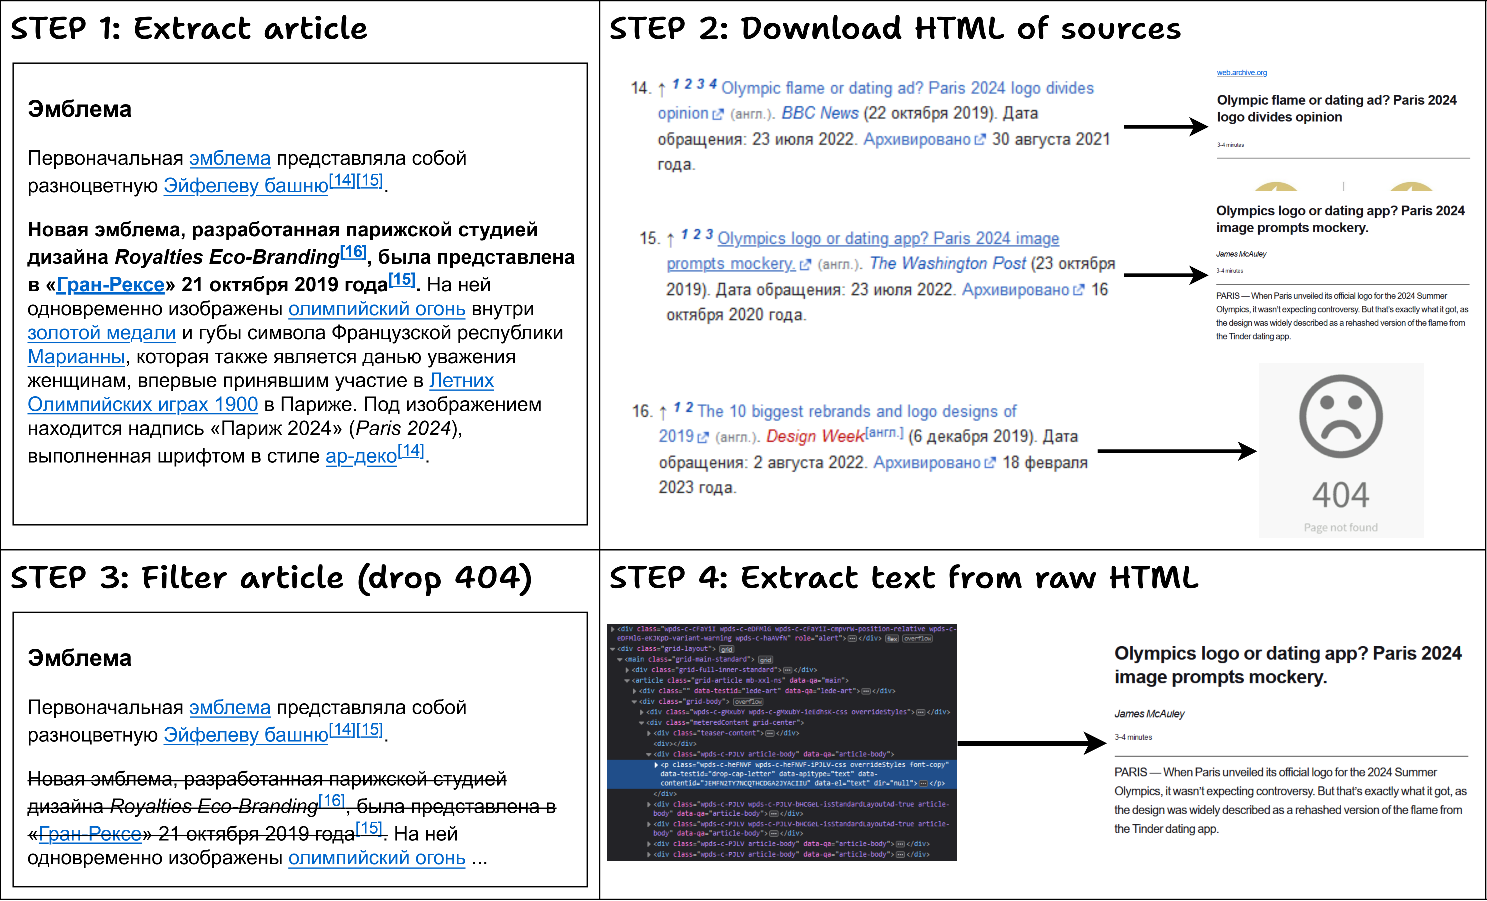
\includegraphics[width=0.8\textwidth]{figures/Source_extract.png}
\caption{Source Extraction}
\label{fig:source}
\end{figure}

\begin{figure}[ht!]
\centering
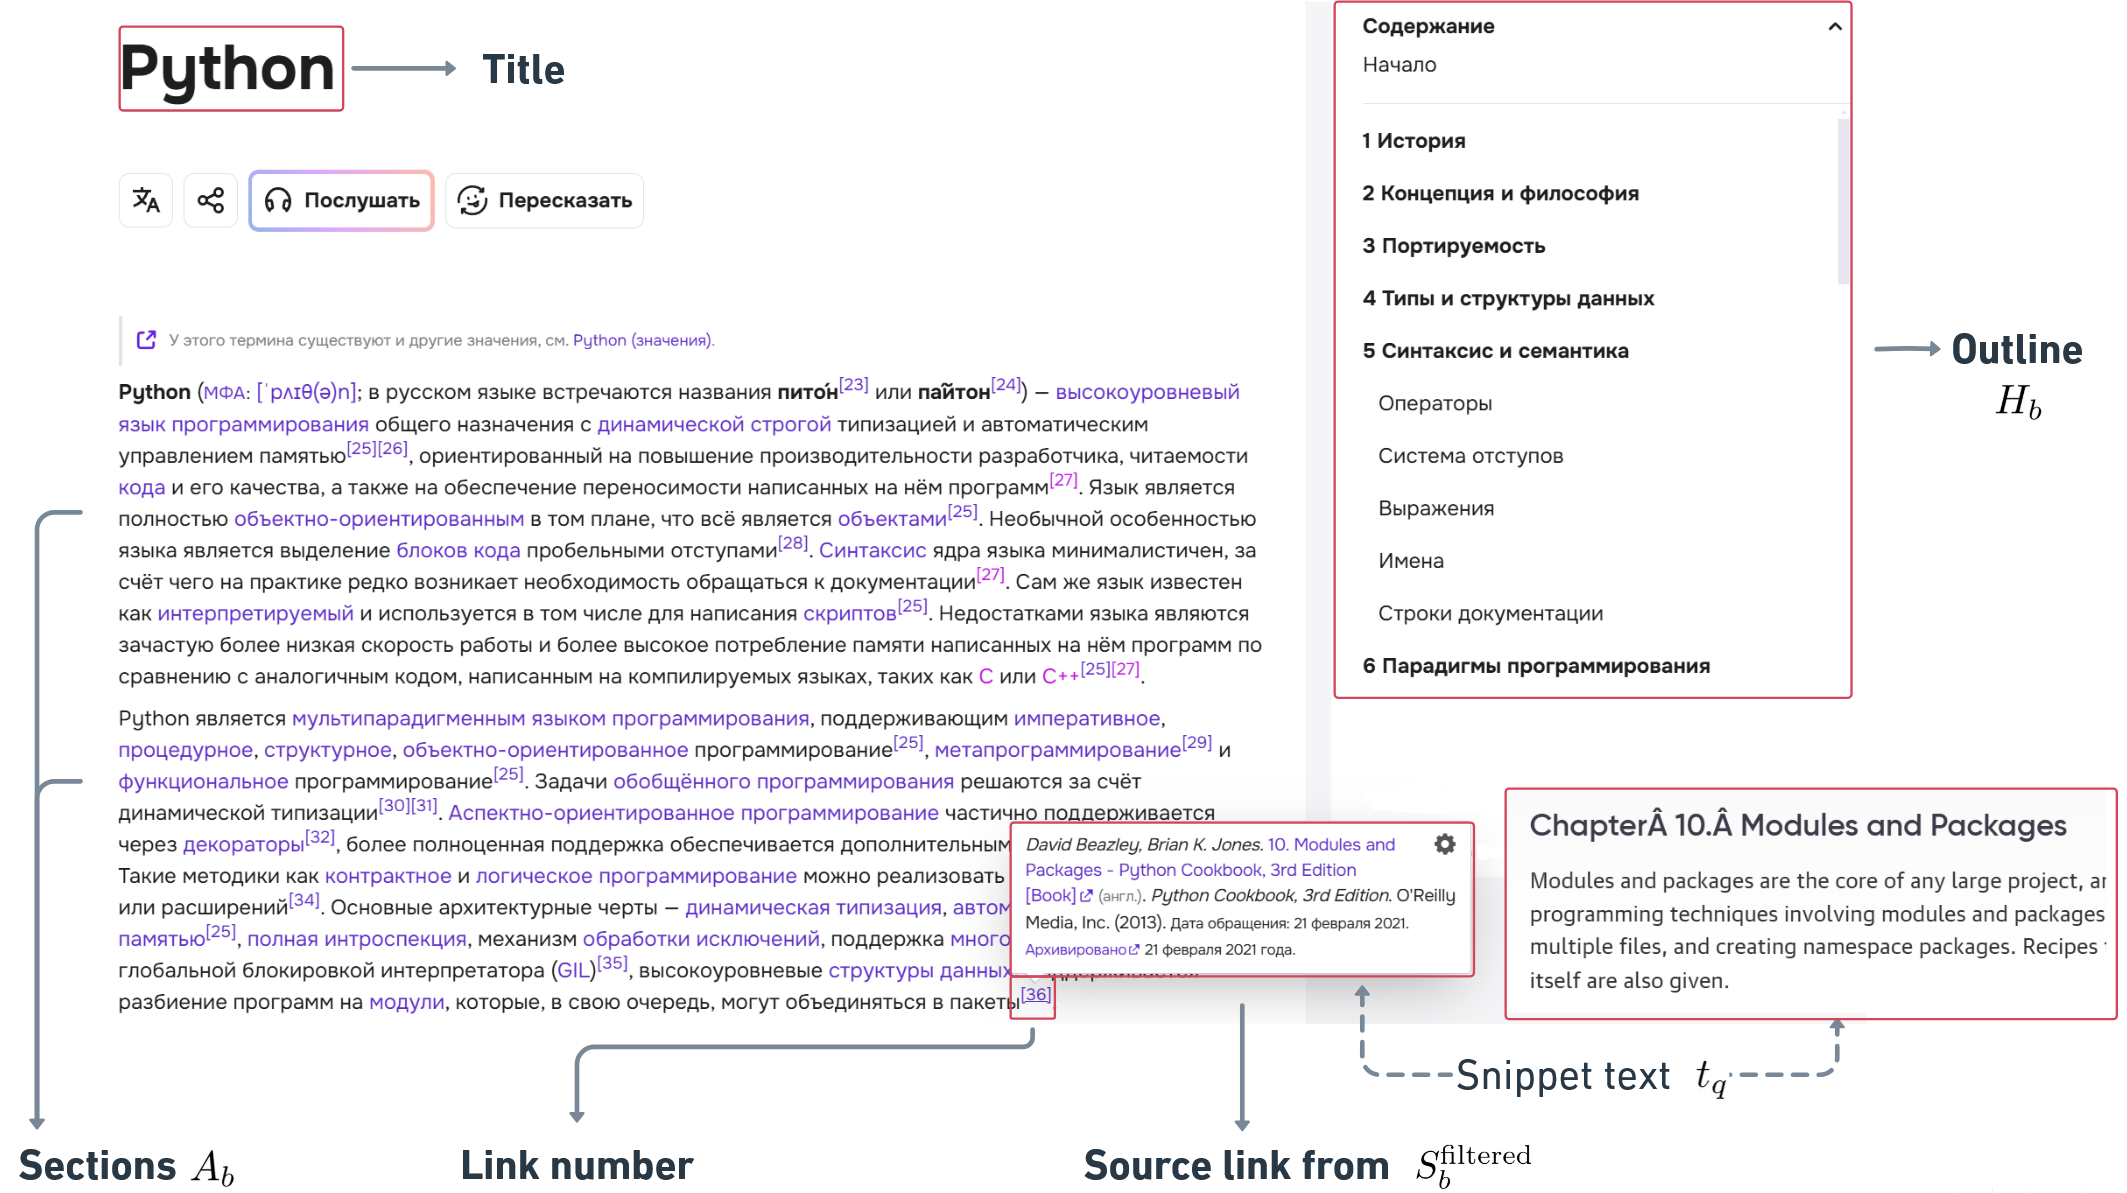
\includegraphics[width=0.8\textwidth]{figures/article_entities.png}
\caption{Main Article Entities}
\label{fig:article}
\end{figure}

During the data acquisition stage, primary information extraction from the selected article and the collection of its associated sources are performed. Figure \ref{fig:source} shows a brief schematic of the source text extraction process. The sources were downloaded using the Python module \texttt{newspaper3k}\footnote{\url{https://github.com/codelucas/newspaper}}.
A subset of "Ruwiki" articles BB is taken as the initial corpus.
The extraction of the article's HTML code is performed using standard Python module tools\footnote{\url{https://beautiful-soup-4.readthedocs.io/en/latest/}}$^,$\footnote{\url{https://requests.readthedocs.io/en/latest/index.html}}.
The obtained text is structured by splitting it into fragments corresponding to nested headings (H1, H2, H3, etc.), which preserves both the substantive part of the article and its hierarchical organization.
Next, all external references cited in the "Notes" section are automatically extracted. Invalid links (e.g., 404 error) are excluded from further processing,
and the text associated with them is removed, leaving only those sources that are actually accessible.

Figure \ref{fig:article} illustrates the schematic breakdown of an article\footnote{\url{https://ru.ruwiki.ru/wiki/Python}} into key entities used in subsequent processing.
During the data processing stage, text filtering is performed to ensure its correct interpretation by the model.
Each footnote (e.g., [1], [2]) is matched to a specific link corresponding to one of the available sources.
This allows for precise identification of the link's position in the article text and its use for subsequent filtering.

\tab{tab:dataset}{Key characteristics of the collected dataset}{
    \begin{tabular}{lcc}
        \hline
        \textbf{Metric} & \textbf{RuWikiBench} & \textbf{ResearchArena} \\
        \hline
        Number of articles & 285 & 7,952 \\
        \hline
        Number of downloaded sources & 15,686 & 12,034,505 \\
        \hline
        Total number of snippets & 36,860 & - \\
        \hline
        Average plan size (number of headings) & 37 & - \\
        \hline
        Average section size (number of words) & 112 & - \\
        \hline
    \end{tabular}
}

Based on the valid links \(S_b^{\mathrm{filtered}}\), filtered sets of paragraphs \(A_b^{\mathrm{filtered}}\) and headings \(H_b^{\mathrm{filtered}}\) are formed.
That is, only content supported by the extracted sources is retained; everything else is removed.
Only sources for which a text \(t_q\) of at least 1500 characters could be retrieved are kept,
to filter out "noisy" responses from HTML pages such as errors (e.g., error 404) or blocking messages.
\(A_b^{\mathrm{filtered}}\) retains only those paragraphs that contain at least one link to a source for which text was successfully retrieved.
Similarly, \(H_b^{\mathrm{filtered}}\) is formed—only those headings under which at least one paragraph remains.
The characteristics of the collected corpus are presented in \tabref{tab:dataset}.

\section{Evaluation Methodology}

To objectively assess the ability of language models to generate scientific and encyclopedic texts, it is necessary to replicate the real process of preparing encyclopedic content:
\begin{enumerate}
    \item \textbf{Selection of relevant sources}: The model is given the article title and a set of snippets, among which it must identify and rank materials relevant to the topic by their significance;
    \item \textbf{Article structure construction}: Based on the topic and selected sources, the model creates an outline with main sections in the Wikipedia style;
    \item \textbf{Section generation}: Article materials are distributed across sections, after which a summary of the relevant materials is generated for each section.
\end{enumerate}
Each stage is evaluated independently of the previous ones, allowing for a quantitative measurement of the quality of each specific subtask.

\subsection{Selection of Relevant Sources}
One of the most effective search strategies \cite{rerank} is the preliminary generation of an expected result (description) based on the original query (article title) to create an expanded search query.
The description is generated in both Russian and English, as the source texts are also available in both languages.
The queries in both languages are then combined into a single textual query for a BM25-based search system.

Experiments were conducted with two approaches to query formulation:
\begin{enumerate}
\item \textbf{Pre-generated query based on the title and second-level headings}: Allows for a clean evaluation of the models' ranking abilities; the LLaMa 3 70b model \cite{llama} was used to generate the query;
\item \textbf{Query generated from the title by the evaluated model}: Similar to real-world conditions, the LLM is fully responsible for the quality of the results and independently decides which search query to formulate for BM25.
\end{enumerate}
Examples of generated descriptions are shown in Figure \ref{fig:cxx}.

\begin{figure}[ht!]
\centering
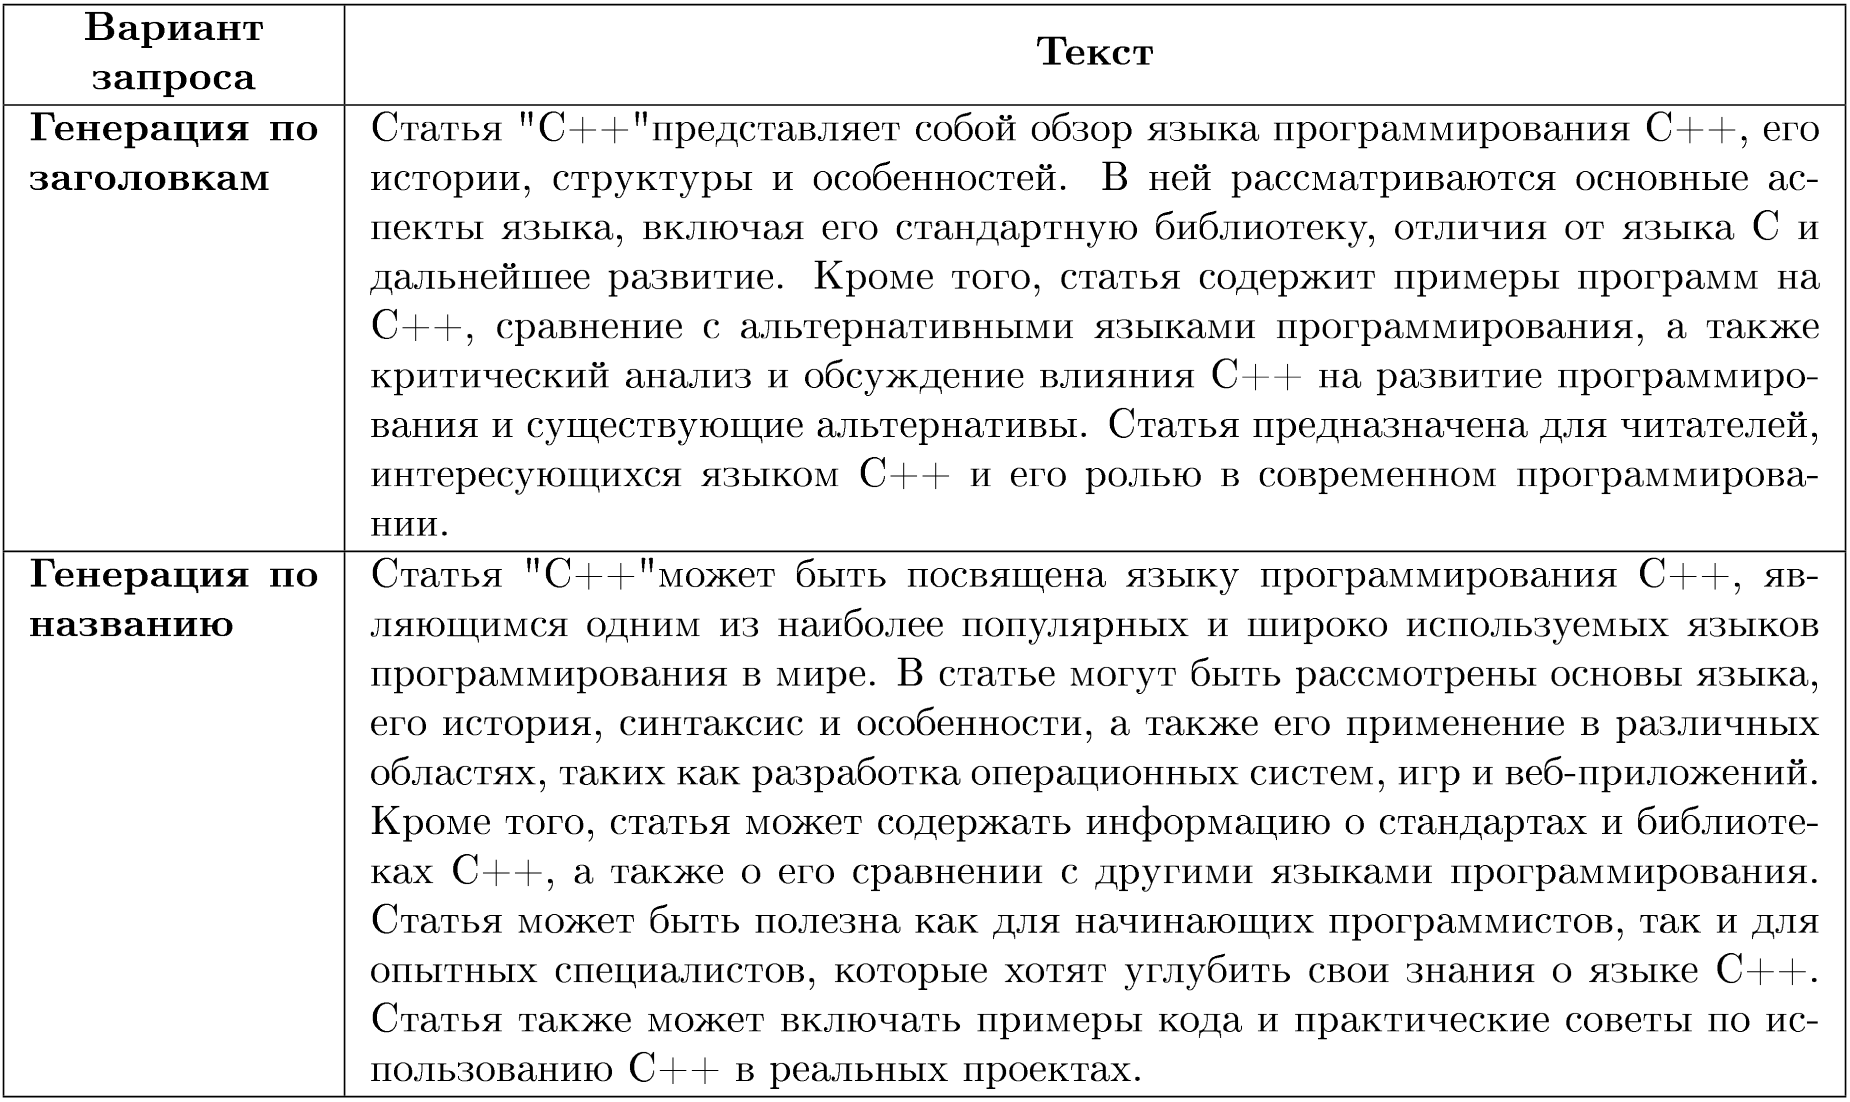
\includegraphics[width=\textwidth]{figures/two_queries.png}
\caption{Comparison of descriptions for the article <<C++>> using the two approaches}
\label{fig:cxx}
\end{figure}

The documents selected by the BM25 query are sequentially passed to the large language model, which must classify each snippet as relevant (answer "yes") or non-relevant (answer "no").
To obtain numerical scores, the titles of the articles to which the retrieved documents belong are compared with the title of the article for which source texts are being selected.
The logarithmic probability of the tokens in the model's response is taken: if the response was affirmative, the probability $P(\text{yes})$ is used; if negative, $1 - P(\text{no})$ is used.
This approach allows ranking the retrieved documents by the model's confidence in their relevance: the higher the probability, the higher the model's confidence in the response, and the higher the document is ranked in the results.

\subsection{Article structure construction}
First, each text fragment (snippet) from the reference article source is converted into a vector representation using a selected embedding model.
Then, the snippets are clustered into potential section contents.
For determinism, the KMeans algorithm is applied with the number of clusters equal to the number of second-level headings in the reference outline, and the centroids are initialized with the vector representations of these headings.

Next, five snippets closest to the cluster center are selected. This is done to reduce the influence of less relevant snippets on the final outline.
The formation of mini-outlines for sections is carried out taking into account two key parameters:
the context window size (to account for references and the overall semantics of the document) and two generation modes — directly from the texts and through preliminary generation of a brief cluster description.
The two generation modes allow for choosing the level of abstraction:
the direct mode preserves details with raw data, while the mode via preliminary cluster description
improves consistency of formulations and reduces information duplication.
At the final stage, all mini-outlines are combined into the final structured article outline.

\subsection{Section generation}
For each article section, all snippets that were indicated as sources for the reference text of the section are extracted.
All snippets are again converted into embeddings, and a pairwise similarity matrix is constructed as the product \(E \times E^\top\).
Elements with a similarity value above the threshold of 0.8 (empirically determined) are considered semantically close and are grouped together to avoid redundant repetitions during generation (e.g., when different sources paraphrase the same information).
For each such semantic group, a hierarchical representation is built: the first five texts are taken, and a brief description is generated based on them.
This description is then supplemented using the next five texts, and so on, until a complete compressed representation of the group is obtained.
Thus, only a set of brief descriptions remains — the most important information without unnecessary repetition.
After this, the text of the section is generated based on the obtained group descriptions using a hierarchical summarization method \cite{hier}.

\section{Experimental Setup Description}
Below is a description of all data, models, hyperparameters, and procedures used to ensure reproducibility and analysis.

\subsection{Generation Parameters}
For all models, unless otherwise specified, the same generation parameters were used: temperature - 0.01, repetition penalty - 1.0, and top\_p - 0.9.

\subsection{Relevant Source Selection}
Snippet indexing was performed using BM25\footnote{\url{https://github.com/xhluca/bm25s}} across the entire corpus of collected snippets without hyperparameter tuning (default values).
For each relevant document, two non-relevant documents were selected (ratio 1:2) — this was done to improve evaluation robustness.

\subsection{Article Structure Construction}
Snippets were converted into vector space using the \texttt{sergeyzh/BERTA}\footnote{\url{https://huggingface.co/sergeyzh/BERTA}} model.
Two context window options were considered: either a zero window (only the snippet itself) or one neighboring snippet to the left and right to expand the context.
Header similarity with reference headers was compared using cosine similarity: semantic correspondence was prioritized over exact wording or header level.
The comparison was performed against the cleaned article structure: all headers whose sections consisted entirely of text without downloadable sources were removed from the preprocessed text.

\section{Evaluation Metrics}

Within the benchmark, two groups of metrics are used: ranking metrics, which assess how well the model selects relevant sources, and text similarity metrics, which measure how closely the generated content matches the reference.

\subsection{Ranking Metrics}

To evaluate the quality of the source list, we use \textbf{NDCG@K} \cite{ndcg} and $\mathrm{R\text{-}Precision}$ \cite{rprecision}:
\begin{equation}\label{ndcg}
\mathrm{NDCG@K}= \frac{\mathrm{DCG@K}}{\mathrm{IDCG@K}}
\end{equation}

\begin{equation}\label{dcg}
\mathrm{DCG@K}= \sum_{i=1}^{K} \frac{\mathrm{rel}_i}{\log_2(i+1)}
\end{equation}

\begin{equation}\label{idcg}
\mathrm{IDCG@K}= \sum_{i=1}^{K} \frac{\mathrm{rel}^{\mathrm{IDEAL}}_i}{\log_2(i+1)}
\end{equation}

\begin{equation}\label{rpr}
\mathrm{R\text{-}Precision}= \frac{\sum_{i=1}^{R} \mathrm{rel}_i}{R}
\end{equation}

where $\mathrm{rel}_i\in\{0,1\}$ is the indicator of relevance for the document at position $i$; $\mathrm{rel}^{\mathrm{IDEAL}}_i$ is the same quantity in the ideal (fully sorted) ranking;
$R$ is the total number of relevant documents for the given query.

\subsection{Text Similarity Metric}
The quality of generated sections and headings is evaluated with \textbf{BERTScore} \cite{bertscore}:

\begin{equation}\label{recall}
R_{\mathrm{BERT}}= \frac{1}{|x|}\sum_{x_i\in x}\max_{\hat{x}_j\in\hat{x}} x_i^\top \hat{x}_j
\end{equation}

\begin{equation}\label{precision}
P_{\mathrm{BERT}}= \frac{1}{|\hat{x}|}\sum_{\hat{x}_j\in\hat{x}}\max_{x_i\in x} x_i^\top \hat{x}_j
\end{equation}

\begin{equation}\label{f}
F_{\mathrm{BERT}}= \frac{2\,P_{\mathrm{BERT}}\,R_{\mathrm{BERT}}}{P_{\mathrm{BERT}} + R_{\mathrm{BERT}}}
\end{equation}

where $x$ is the reference text, $\hat{x}$ is the generated text; each sentence is encoded using the model\footnote{\url{https://huggingface.co/sergeyzh/BERTA}}, after which cosine similarity is computed.

We also considered ROUGE-\allowbreak L and BLEU for evaluating section generations.

\textbf{ROUGE-L} \cite{rouge} is based on the length of the longest common subsequence (LCS) between the generated summary $S$ and the reference $R$:
\begin{equation}\label{r_p}
  \text{Precision} = \frac{\mathrm{LCS}(S,R)}{|S|},\quad
\end{equation}
\begin{equation}\label{r_r}
  \text{Recall} = \frac{\mathrm{LCS}(S,R)}{|R|}
\end{equation}
\begin{equation}\label{rouge}
  \text{ROUGE‑L} = \frac{2\;\text{Precision}\;\cdot\;\text{Recall}}{\text{Precision} + \text{Recall}}
\end{equation}

\textbf{BLEU} \cite{bleu} is an n-gram precision metric with a brevity penalty. The final score is given by Equation \eqref{bleu}:
\begin{equation}\label{bleu}
\mathrm{BLEU}_N = \mathrm{BP}\cdot \exp\!\left(\sum_{n=1}^{N} w_n \log p_n\right),
\end{equation}
where $p_n$ is the precision for $n$-grams, $w_n$ are the weights, and $\mathrm{BP}$ is the brevity penalty.


\section{Description of Experimental Results}

\subsection{Models}
The experiments used the following large language models:
RuadaptQwen2.5-\allowbreak 7B-\allowbreak Lite-\allowbreak Beta \cite{ruadapt},
RuadaptQwen3-\allowbreak 32B-\allowbreak Instruct-\allowbreak v2 \cite{ruadapt}, 
DeepSeek V3 \cite{deepseek}, 
Qwen3-\allowbreak 235B-\allowbreak A22B \cite{qwen3}, 
tpro \cite{tpro} and yagpt5lite \cite{yagpt}.
In all tables, models are ordered by size, and the best results within each parameter group are highlighted.

\subsection{Results}
Tables \ref{tab:query_ref} and \ref{tab:query_def} present the results of measuring ranking quality.
We also include baseline results, represented by BM25 retrieval without model-based reranking.
In the first case (Table \ref{tab:query_ref}), where a pre-generated search query was used for all models,
the best results were achieved by DeepSeek V3, which indicates a strong ability to select relevant documents.
In the second experiment (\ref{tab:query_def}), where the query was formed solely from the article title, tpro achieved the best results.
The experiment showed that BM25’s own query generation is not inferior in ranking quality to the reference setup, in which queries are generated by a more “powerful” model and then
used by all evaluated models. Presumably, this is because—as shown in Figure \ref{fig:cxx}—the queries turn out to be similar:
LLMs have knowledge of Wikipedia’s typical article structure from training and can therefore connect relevant concepts in the required format.

\begin{table}[ht!]
\centering
\caption{Results of pure ranking ability evaluation}
\begin{tabular}{l|c|c}
\hline
\textbf{Model} & \textbf{NDCG} & \textbf{R-Pr} \\
\hline
baseline (bm25)                                                  & 88.81 & 62.51 \\
\hline
\textbf{DeepSeek V3}                                             & \uline{\textbf{95.42}} & \uline{\textbf{83.86}} \\
Qwen3-\allowbreak 235B-\allowbreak A22B                          & 94.49 & 82.42 \\
\hline
RuadaptQwen3-\allowbreak 32B-\allowbreak Instruct-\allowbreak v2 & 95.25 & 81.81 \\
tpro                                                             & \uline{95.42} & \uline{83.53} \\
\hline
RuadaptQwen2.5-7B-\allowbreak Lite-\allowbreak Beta              & 88.26 & 62.26 \\
yagpt5lite                                                       & \uline{90.35} & \uline{77.66} \\
\hline
\end{tabular}
\label{tab:query_ref}
\end{table}

\begin{table}[ht]
\centering
\caption{Results of evaluating BM25 query-generation ability}
\begin{tabular}{l|cc|cc}
\hline
\multirow{2}{*}{\textbf{Model}} & \multicolumn{2}{c|}{\textbf{BM25}} & \multicolumn{2}{c}{\textbf{Rerank}} \\
& \textbf{NDCG} & \textbf{R-Pr} & \textbf{NDCG} & \textbf{R-Pr} \\
\hline
DeepSeek V3                                                      & 88.39 & 60.65 & \uline{95.67} & \uline{83.07} \\
Qwen3-235B-A22B                                                  & \uline{89.17} & \uline{62.98} & 94.90 & 81.96 \\
\hline
RuadaptQwen3-\allowbreak 32B-\allowbreak Instruct-\allowbreak v2 & 85.39 & 52.80 & 95.82 & 81.62 \\
\textbf{tpro}                                                    & \uline{\textbf{90.61}} & \uline{\textbf{65.07}} & \uline{\textbf{96.06}} & \uline{\textbf{83.37}} \\
\hline
RuadaptQwen2.5-7B-\allowbreak Lite-\allowbreak Beta              & \uline{88.81} & \uline{62.51} & 88.23 & 60.96 \\
yagpt5lite                                                       & 86.59 & 57.98 & \uline{90.27} & \uline{77.65} \\
\hline
\end{tabular}
\label{tab:query_def}
\end{table}

Overall, the models show fairly high metric values at this stage, which may be due to the fact that an article title reflects its content well.
In the best cases, up to 80\% of the documents in the sample are relevant, which can be considered a good figure; however, there remains potential for further improvement.

\begin{table}[ht!]
\centering
\caption{Results of outline generation}
\begin{tabular}{l|c|c|c}
\hline
\multirow{2}{*}{\textbf{Model}} & \multicolumn{3}{c}{\textbf{Mean BERTScore F1}} \\
\cline{2-4}
& \multicolumn{2}{c|}{\textbf{Direct}} & \multirow{2}{*}{\textbf{Description}} \\
\cline{2-3}
& \textbf{no neighbors} & \makecell{\textbf{one neighbor}} & \\
\hline
\textbf{DeepSeek V3}                                             & \uline{\textbf{63.51}} & \uline{\textbf{62.93}} & \uline{\textbf{65.50}} \\
Qwen3-\allowbreak 235B-\allowbreak A22B                          & 60.86 & 59.06 & 62.66 \\
\hline
RuadaptQwen3-\allowbreak 32B-\allowbreak Instruct-\allowbreak v2 & 60.12 & \uline{60.04} & \uline{62.91} \\
tpro                                                             & \uline{60.32} & 59.09 & 60.75 \\
\hline
RuadaptQwen2.5-7B-\allowbreak Lite-\allowbreak Beta              & \uline{60.03} & 58.21 & \uline{61.58} \\
yagpt5lite                                                       & 59.72 & \uline{60.07} & 60.25 \\
\hline
\end{tabular}
\label{tab:outline_res}
\end{table}

Table \ref{tab:outline_res} presents the results of evaluating article-structure construction.
Direct — generation from the cluster snippets, with neighbor context as indicated; Description — generation via a preliminary description of all cluster elements.
The results show that with preliminary description generation, all models consistently improve in quality.
RuadaptQwen3 shows the largest gain, rising to second place and effectively matching the results of the larger model,
Qwen3-\allowbreak 235B-\allowbreak A22B. DeepSeek V3 remains the leader, showing a substantial margin over the others. At the bottom in quality are RuadaptQwen2.5-7B-\allowbreak Lite-\allowbreak Beta and yagpt5lite.
At the same time, yagpt5lite, with only 8 billion parameters, delivers results comparable to a 32-billion-parameter model.
Figure \ref{fig:outline} shows a comparison of a small excerpt of the reference and generated outlines.
The obtained results correlate well with the degree of similarity between the headings and the reference. A common issue across all models was excessive heading hierarchy depth.
On “Ruviki”, headings were rarely deeper than level three; however, the models often created fourth- and fifth-level headings, implying that all information belongs in one large section,
even though it may differ somewhat in meaning and, in the original outline, would correspond to unrelated headings.

\begin{figure}[ht!]
\centering
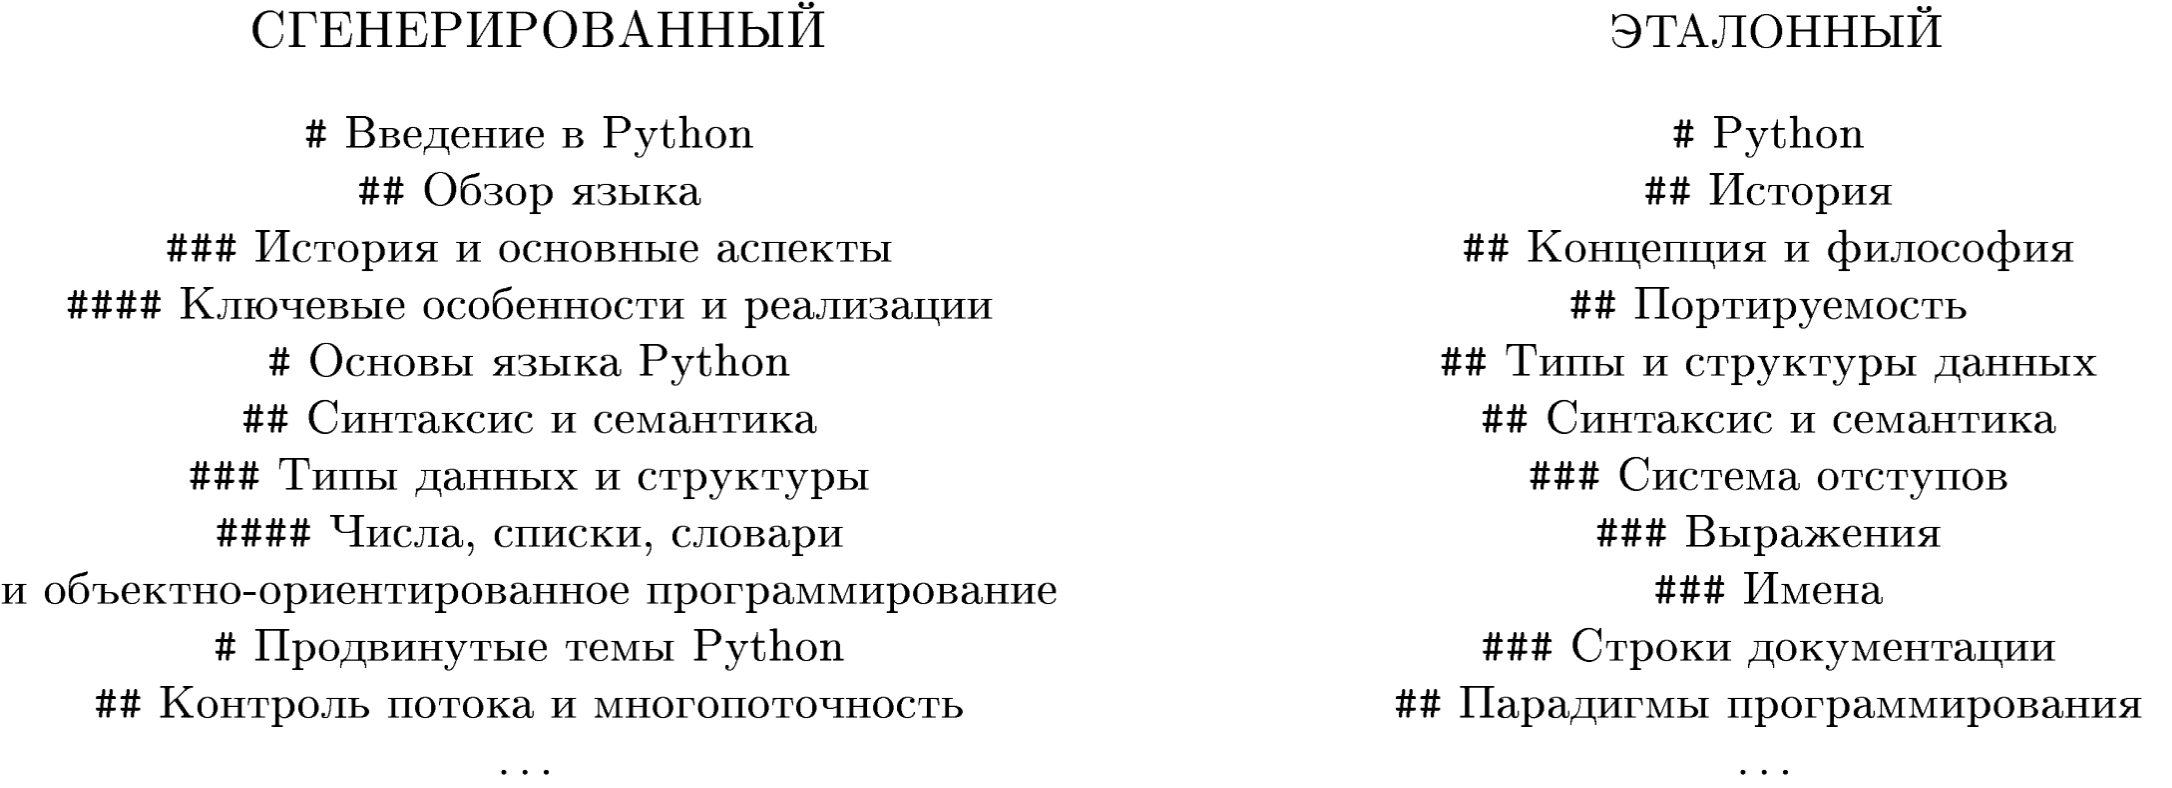
\includegraphics[width=\textwidth]{figures/outline.png}
\caption{Comparison of two article outlines}
\label{fig:outline}
\end{figure}

Table \ref{tab:secs} reports the measurements of section-generation quality. The final results are at roughly the same level, but this is due to the sensitivity of the metric used.
Sections for which the algorithm did not select a single relevant snippet were excluded from the final metrics. The best overall results
were demonstrated by Qwen3-\allowbreak 235B-\allowbreak A22B; however, in terms of ROUGE-\allowbreak L and BLEU, RuadaptQwen3-\allowbreak 32BInstruct-v2 leads, indicating better structural consistency and
greater overlap of wording with the reference.
The yagpt5lite model performs above average—especially on BLEU—at a much smaller size, whereas tpro shows the lowest values across all metrics.

\begin{table}[ht!]
\centering
\caption{Results of section generation}
\begin{tabular}{l|c|c|c}
\hline
\textbf{Model} & \textbf{Mean F1} & \textbf{Mean ROUGE-L} & \textbf{Mean BLEU} \\
\hline
DeepSeek V3                                                               & 53.48 & 14.34 & 2.81 \\
Qwen3-\allowbreak 235B-\allowbreak A22B                                   & \uline{\textbf{53.74}} & \uline{14.63} & \uline{3.07} \\
\hline
\textbf{RuadaptQwen3-\allowbreak 32B-\allowbreak Instruct-\allowbreak v2} & 53.21 & \uline{\textbf{15.46}} & \uline{\textbf{3.40}} \\
tpro                                                                      & 53.15 & 13.58 & 2.27 \\
\hline
RuadaptQwen2.5-7B-\allowbreak Lite-\allowbreak Beta                       & 52.99 & 12.29 & 2.11 \\
yagpt5lite                                                                & \uline{53.43} & \uline{14.85} & \uline{3.16} \\
\hline
\end{tabular}
\label{tab:secs}
\end{table}

For a visual comparison of section-generation quality, consider the introductory parts of the article “COVID19”
produced by DeepSeek V3 and yagpt5lite, respectively, shown in Figure \ref{fig:secs_com}.
Despite some semantic inaccuracies (for example, the statement “COVID-19 is a pandemic,” whereas in reality it is a disease),
yagpt5lite demonstrates a quite solid result. Its text falls short of DeepSeek V3’s version in terms of coverage and systematic exposition,
but contains more numerical data and concrete facts. At the same time, the material generated by DeepSeek V3 reads like an excerpt from an encyclopedic article,
whereas the yagpt5lite version is closer in style to a technical report on the disease.

\begin{figure}[ht!]
\centering
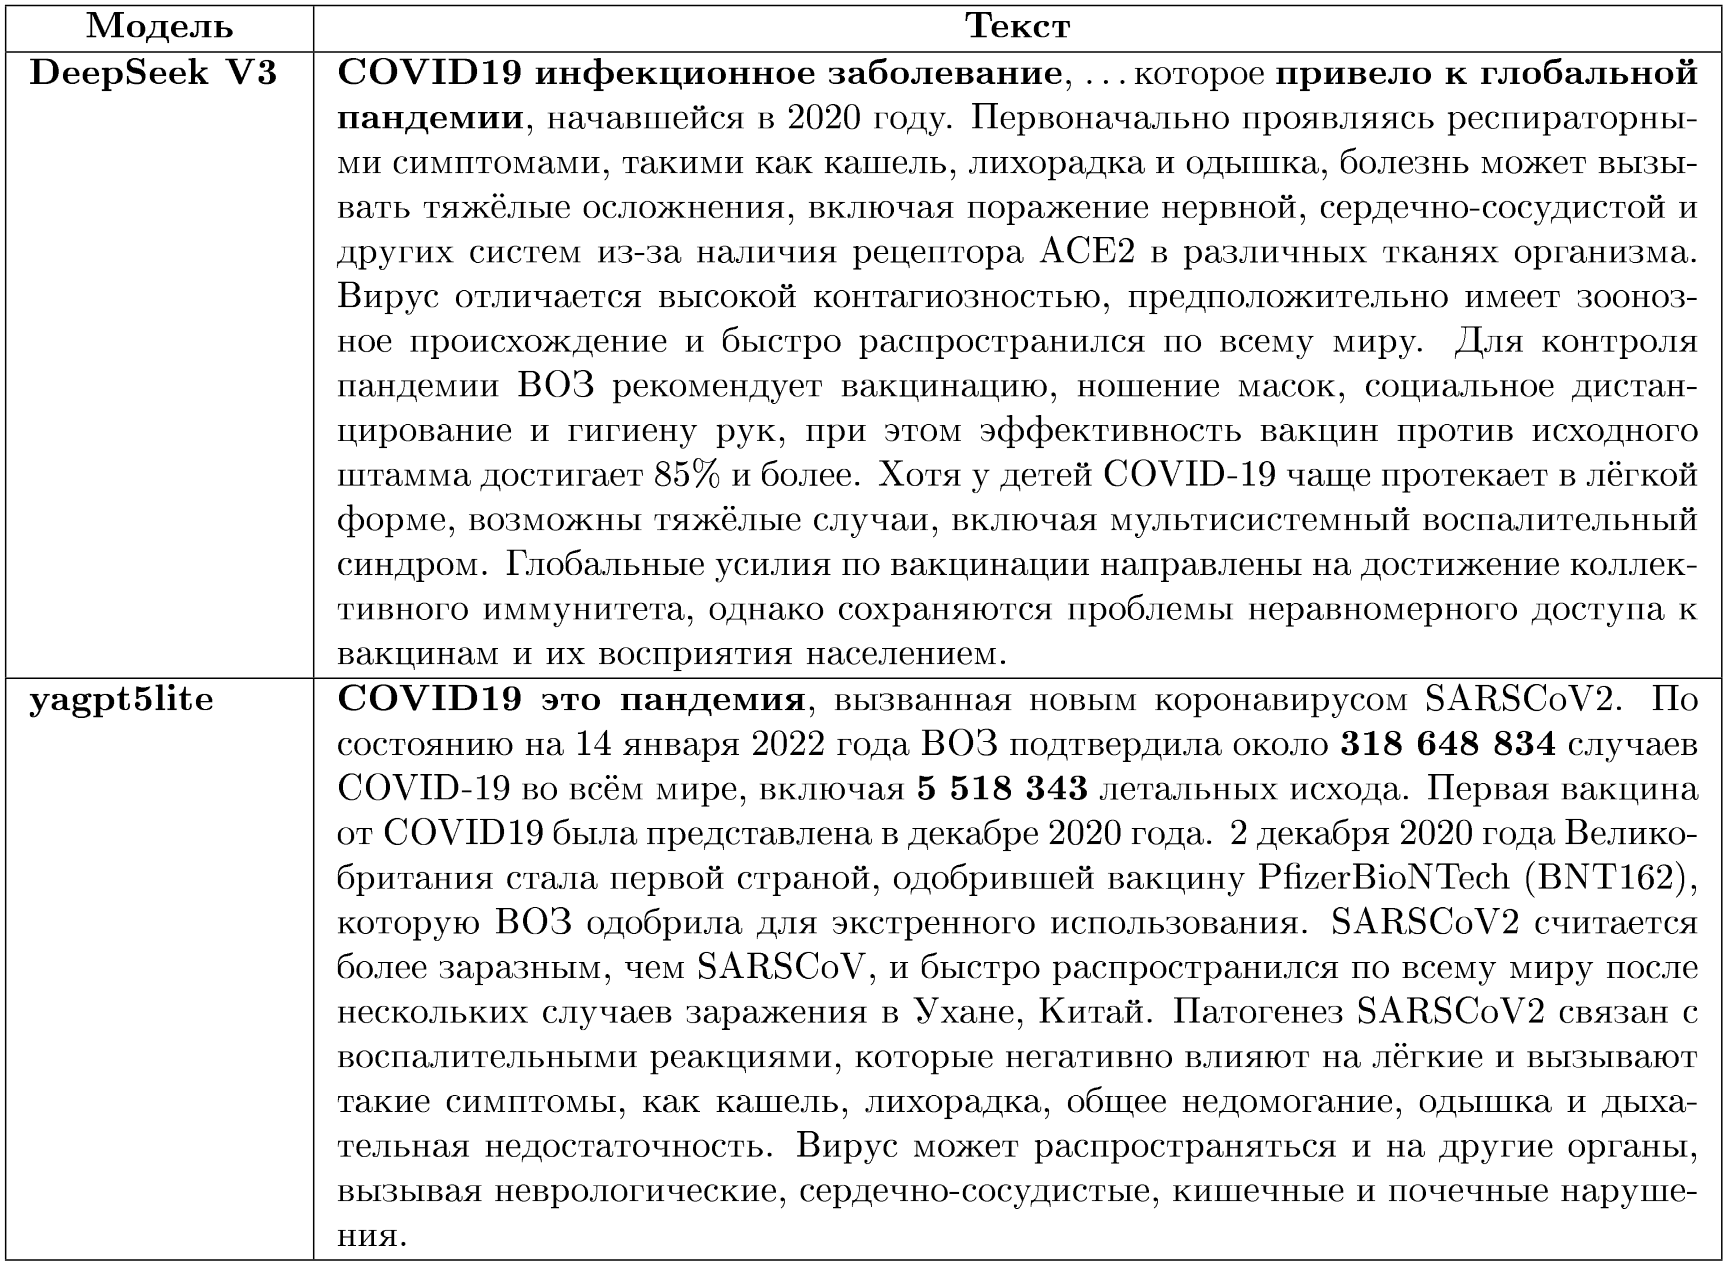
\includegraphics[width=0.9\textwidth]{figures/two_secs.png}
\caption{Comparison of two section texts}
\label{fig:secs_com}
\end{figure}

\section*{Conclusion}
This paper proposes and implements the RuWikiBench benchmark for evaluating the analytical capabilities of large language models in generating scientific and encyclopedic texts in Russian. 
The core of the proposed evaluation system is a three-stage process, consisting of three independent systems that naturally arise when creating articles on a specific topic. 
Relying on a filtered "Ruwiki" corpus with aligned snippets and a clearly defined evaluation methodology, the proposed benchmark establishes a foundation for further research in the application of language models to the 
task of generating scientific and encyclopedic text.

Experiments showed that with a fixed search query, DeepSeek V3 demonstrates the best source selection quality, significantly outperforming BM25 without reranking. 
At the structure construction stage, it was found that adding a preliminary cluster description consistently improves the quality of outlines for all models, 
including DeepSeek V3, which demonstrated the best understanding of the process. All models showed comparable text generation quality; 
however, RuadaptQwen3-\allowbreak 32B-\allowbreak Instruct-\allowbreak v2 leads in ROUGE-L and BLEU metrics, indicating a text structure more consistent with the reference. 
The work shows that models possess significant potential, but their reliable application requires further development of methods for analyzing and structuring review materials.

\section*{Acknowledgements}
The study was supported by grant No. 25-11-00191 from the Russian Science Foundation.
The work was carried out using the supercomputer "MSU-270" of the Lomonosov Moscow State University.



\bibliographystyle{superfri}
\begin{thebibliography}{99}

\bibitem{rsglue}
\textit{RussianSuperGlue.}
Shavrina, Tatiana, et al. "RussianSuperGLUE: A Russian Language Understanding Evaluation Benchmark." Proceedings of the 2020 Conference on Empirical Methods in Natural Language Processing (EMNLP). 2020.

\bibitem{mera}
\textit{Mera.}
Fenogenova, Alena, et al. "MERA: A Comprehensive LLM Evaluation in Russian." Proceedings of the 62nd Annual Meeting of the Association for Computational Linguistics (Volume 1: Long Papers). 2024.

\bibitem{libra}
\textit{LIBRA.}
Churin I. et al. Long Input Benchmark for Russian Analysis //CoRR. – 2024.

\bibitem{arena}
VikhrModels. RuLLM Arena: Russian LLM Evaluation Benchmark // GitHub repository. – URL: \url{https://github.com/VikhrModels/ru_llm_arena} (accessed: 01.08.2025).

\bibitem{pp}
\textit{Ping-Pong.}
Gusev I. PingPong: A Benchmark for Role-Playing Language Models with User Emulation and Multi-Model Evaluation.

\bibitem{deepr}
\textit{OpenAI.}
Introducing deep research // OpenAI URL: \url{https://openai.com/index/introducing-deep-research/} (accessed: 31.07.2025).

\bibitem{storm}
\textit{Storm.}
Shao Y. et al. Assisting in Writing Wikipedia-like Articles From Scratch with Large Language Models //NAACL-HLT. - 2024

\bibitem{resar}
\textit{ResearchArena.}
Kang, Hao, and Chenyan Xiong. "ResearchArena: Benchmarking LLMs' Ability to Collect and Organize Information as Research Agents." arXiv e-prints (2024): arXiv-2406.

\bibitem{rerank}
\textit{Reranking.}
Wang X. et al. Searching for Best Practices in Retrieval-Augmented Generation //CoRR. - 2024.

\bibitem{llama}
Touvron H. et al. LLaMA: Open and Efficient Foundation Language Models.

\bibitem{hier} 
Wu, Jeff, et al. "Recursively summarizing books with human feedback." arXiv preprint arXiv:2109.10862 (2021).

\bibitem{ndcg}
\textit{NDCG.}
Järvelin, Kalervo, and Jaana Kekäläinen. "Cumulated gain-based evaluation of IR techniques." ACM Transactions on Information Systems (TOIS) 20.4 (2002): 422-446.

\bibitem{rprecision}
\textit{R-Precision.}
BUCKLEY C. Evaluating Evaluation Measure Stability //ACM SIGIR 2000 Proceedings. - 2000.

\bibitem{bertscore}
\textit{BERTScore.}
Zhang T. et al. BERTScore: Evaluating Text Generation with BERT //International Conference on Learning Representations.

\bibitem{rouge}
\textit{ROUGE.}
Lin, Chin-Yew. "Rouge: A package for automatic evaluation of summaries." Text summarization branches out. 2004.

\bibitem{bleu}
\textit{BLEU.}
Papineni K. et al. BLEU: a Method for Automatic Evaluation of Machine Translation.

\bibitem{ruadapt}
\textit{RuadaptQwen.}
Tikhomirov, Mikhail, and Daniil Chernyshev. "Facilitating large language model russian adaptation with learned embedding propagation." Journal of Language and Education 10.4 (40) (2024): 130-145.

\bibitem{deepseek}
\textit{DeepSeek V3.}
Liu A. et al. DeepSeek-V3 Technical Report //CoRR. - 2024.

\bibitem{qwen3}
\textit{Qwen3-\allowbreak 235B.}
Yang A. et al. Qwen3 technical report //arXiv preprint arXiv:2505.09388. - 2025.

\bibitem{tpro}
T-Bank has opened access to its own Russian-language language model in the weight category of 7-8 billion parameters / T-Bank URL: \url{https://www.tbank.ru/about/news/20072024-t-bank-opened-access-its-own-russian-language-language-model-weight-category-of-7-8-billion-parameters/} (accessed: 10.05.2025).

\bibitem{yagpt}
YandexGPT 5 with reasoning mode // Yandex URL: https://ya.ru/ai/gpt (accessed: 30.07.2025).

\end{thebibliography}
\end{document}